\chapter{Evaluation}
In this chapter I outline my findings using tables and graphs where appropriate.
An analysis of the corpus and the tests conducted to tweak the model parameters is presented.
The analysis of the temporal performance is then presented.
The temporal performance for building the models and the temporal performance for conducting document similarity queries will be presented.
The quality of the recommendations will then be analysed.
The quality will be evaluated using two criteria; comparison against the arXiv defined topic groupings and a manual evaluation of the document results.

\section{Corpus Analysis}
In this section an analysis of the arXiv corpus is presented.
The number of words or features present in the corpus are evaluated using a number of different filtering techniques.
The filtering technique used in the later evaluations will be compared against the other filtering techniques considered.

\subsection{Corpus Features}
The arXiv corpus consists to 50,400 documents from a number of arXiv topic groupings.
A breakdown of the groupings can be found in Table~\ref{table:arxivBreakdown}.
Approximately 30,000 of the papers are related to astrophysics, condensed matter and high energy physics.
The bias towards those topics may influence the models generated.
The removal of frequent and infrequent terms from the corpus will be presented below.
I believed originally that filtering out very frequent terms could have had a negative effect on the dictionaries generated.
As the aforementioned groupings make up approximately 60\% of the corpus, I believed filtering could possibly remove words common to those papers.
As show in Table~\ref{table:frequentFeatures}, filtering out very common words had very little impact on the overall size of the corpus feature space.

\begin{table}[h]
    \centering
    \begin{tabular}{|c c|}
         \hline
         arXiv Topics & Number Documents \\ [0.5ex]
         \hline\hline
         astro-ph & 10572 \\
         cond-mat & 10262 \\
         hep-ph & 6770 \\
         hep-th & 5226 \\
         math & 4968 \\
         quant-ph & 2634 \\
         gr-qc & 2073 \\
         nucl-th & 1563 \\
         physics & 1511 \\
         hep-ex & 1257 \\
         nlin & 1120 \\
         math-ph & 815 \\
         hep-lat & 703 \\
         cs & 588 \\
         nucl-ex & 338 \\ [0.5ex]
         \hline\hline
         Total & 50400\\ [1ex]
         \hline
    \end{tabular}
    \caption{Breakdown of papers from arXiv topics}
    \label{table:arxivBreakdown}
\end{table}

Using all 50,000 arXiv documents with no filtering applied, there are 1,520,730 unique tokens in the corpus dictionary.
A large number of these features appear in only a small number of the documents (possibly noise caused by errors in the source document) or they appear in the majority of the documents.
Both of these can cause problems when creating the models.
A word that appears very few times in all of the documents is going to have very little impact on the quality of the models created.
This can lead to a very sparse feature space as each word vector will contain mostly zero entries.
By filtering out these infrequent terms we can reduce the feature space and make our models more efficient by making our vectors less sparse. The following is an analysis of the size of the feature space as different filtering strategies were applied to the corpus.

\begin{figure}[h]
    \centering
        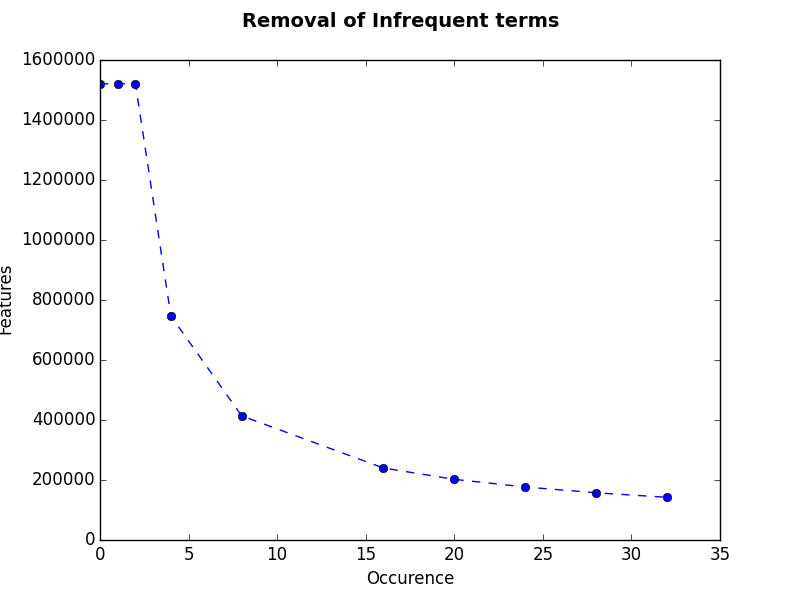
\includegraphics[width=0.7\textwidth]{Figures/CorpusFilterInfrequent.png}
    \caption{Feature space as infrequent words removed}
    \label{fig:FilterInfrequent}
\end{figure}

\begin{table}[h]
    \centering
    \begin{tabular}{|c c|}
         \hline
         Min Occurrences & Number Features \\ [0.5ex]
         \hline\hline
         0 & 1520730 \\
         1 & 1520730 \\
         2 & 1520730 \\
         4 & 746866 \\
         8 & 413733 \\
         16 & 239986 \\
         20 & 202237 \\
         24 & 176699 \\
         28 & 157388 \\
         32 & 142357 \\ [1ex]
         \hline
    \end{tabular}
    \caption{Number of feature as infrequent words filtered}
    \label{table:infrequentFeatures}
\end{table}

In Figure~\ref{fig:FilterInfrequent} we can see that as we filter out infrequent words the size of the feature space shrinks dramatically until we reach words that are in at least 20 documents.
The rate the corpus shrinks seems to level off at around 20-30 documents.
By filtering words using this strategy it was hoped that words which would be considered as noise would be removed from the dataset.

For each of the filtered dictionaries, a list of words whose frequency was one greater than the filter amount, was manually examined.
From my analsis of the sample features a large number appeared to be random unicode characters, parts of mathematical equations or incomprehensible words.
An example of some of the words can be seen in Table ~\ref{table:infrequentWords}:

\begin{table}[h]
    \centering
    \begin{tabular}{|c c|}
         \hline
         Min Occurrences & Sample Words \\ [0.5ex]
         \hline\hline
         1 &  43+6, e−ih(tk, éri\\
         2 &  weiskopf9, 43+3, e−ih(t1\\
         4 &  (yt), nalysis, talbi\\
         8 &  82.70.-y, morsesmale, (1975\\
         16 &  ω(xf, 29.87, dnq\\
         20 &  5-ghz, 0.5-0.6, dolag\\
         24 &  δ(ei, (msd), pseudoclassical\\
         28 &  fic, thorlacius, ha3\\
         32 &  devriendt, hyung, fib\\ [1ex]
         \hline
    \end{tabular}
    \caption{Sample words removed from corpus}
    \label{table:infrequentWords}
\end{table}

\begin{figure}[h]
    \centering
        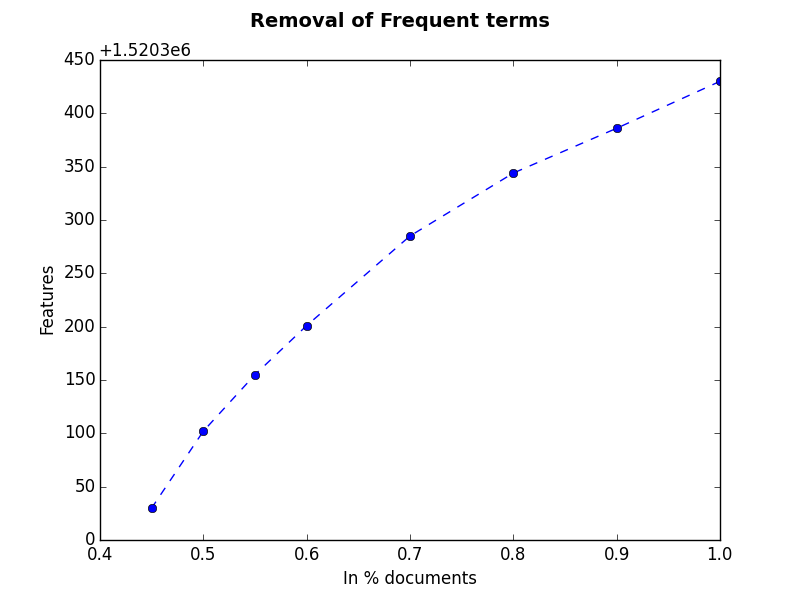
\includegraphics[width=0.7\textwidth]{Figures/CorpusFilterFrequent.png}
    \caption{Feature space as frequent words removed}
    \label{fig:FilterFrequent}
\end{figure}

\begin{table}[h]
    \centering
    \begin{tabular}{|c c|}
         \hline
         Percentage Occurrences & Number Features \\ [0.5ex]
         \hline\hline
         100 & 1520730 \\
         90 & 1520686 \\
         80 & 1520644 \\
         70 & 1520585 \\
         60 & 1520501 \\
         55 & 1520455 \\
         50 & 1520402 \\
         45 & 1520330 \\ [1ex]
         \hline
    \end{tabular}
    \caption{Number of feature as frequent words filtered}
    \label{table:frequentFeatures}
\end{table}

In Figure~\ref{fig:FilterFrequent} we can see the effects of filtering out words which appear in a large percentage of the documents in the corpus.
Compared to the filtering of infrequent terms shown previously, the filtering of frequent terms seems less effective.

These words are very likely to be words that would be very common English words such as "the", "and", "but", "a", "if", "or", etc.
These words are filtered from the corpus as they are so common in the documents that they are not distinguishable features that could be used to separate papers into different groupings.

From the above analysis of above analysis of filtering the corpus, it was decided that terms that appeared in less than 20 of the documents or appeared in at least 75\% of the documents would be filtered out.
The lower bound of 20 was decided upon, as the number of features removed from the dictionary appeared to level off at around 20-25 minimum occurrences.
It was found that filtering out very frequent words had very little effect on the size of the dictionary.
The filter of 75\% was decide upon in order to remove very common words that could also have been removed using a list of stop-words.

\subsection{LDA Topic coherrency}
In this section the arXiv corpus was analysed by examining the quality of topics generated.
For this analyse a sample of 3000 papers from the arXiv corpus was selected and the number of topics varied in multiples of 50 from 50-300.
The topics generated by the LDA algorithm were then manually evaluated.
This range was chosen based on the experiments conducted by Blei on the Nature corpus and an a different corpus of arXiv documents.
It was found that generating models with 100 topics seemed to generate the most coherent topics.

Until version 0.11 of Gensim, the coherence of LDA topics was analysed by manually evaluating the topics generated.
In version 0.11 of Gensim a function was added to sort topics based on their coherence.
This was based on the work of Mimno in his 2011 paper for evaluating the coherence of LDA topics.
Unfortunately this update was released too late into the project to be used in the evaluation of LDA topics.
Future work into this research could use this functionality when choosing the number of LDA topics to use.

\section{Temporal Performance}
The temporal performance can be split into two sections; the time taken to build the models and the time take to run similarity queries on the models.

\subsection{Building Models}
The building of the models can be split into two stages;
the preprocessing of the corpus and then the training of the models.

Due to the differences in the three algorithms being evaluated, the time to preprocess the LDA and k-NN models will be naturally greater than Word2Vec.
This is due to the LDA and k-NN algorithms requiring a bag-of-words representation of the corpus.
First the corpus dictionary must be created by passing over the corpus once and the dictionary filtered of frequent or infrequent terms.
The corpus must then be passed over once more to translate each document into a bag-of-words representation.

Word2Vec on the other hand trains it's model on the textual representation of the corpus and doesn't require any extra preprocessing.
For this reason the time to preprocess LDA and k-NN is presented in Figure~\ref{fig:BuildBow}.

\begin{figure}[h]
    \centering
        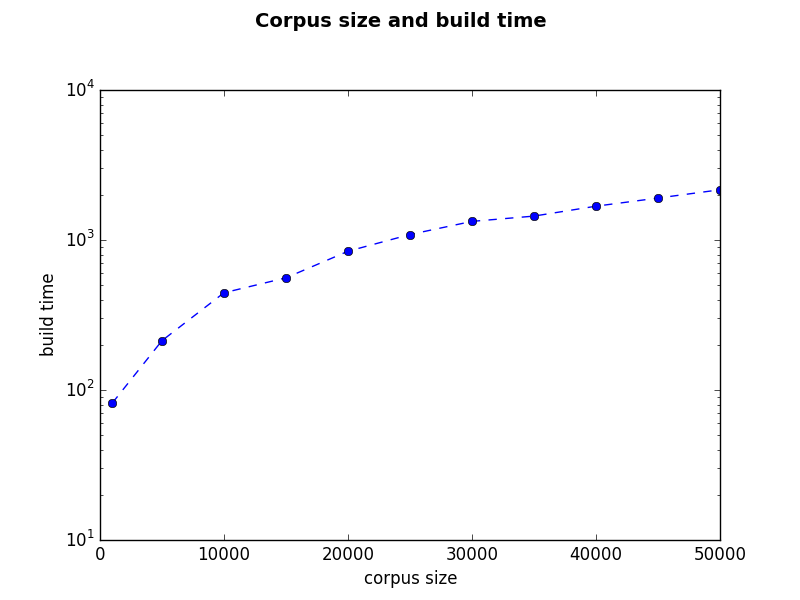
\includegraphics[width=0.7\textwidth]{Figures/BuildBOW.png}
    \caption{Time to preprocess LDA and k-NN}
    \label{fig:BuildBow}
\end{figure}

The time taken to train LDA, k-NN and Word2Vec is presented in Figure~\ref{fig:TrainAll}.
It should be noted that k-NN stops functioning at a corpus of approximately 35,000 documents.
This is due to the the underlying C++ library causing a segmentation fault as the size of the corpus increases.
This is possibly caused by the machine the models were being built on running out of memory.
When training a corpus of 30,000 documents it was noted that the process had allocate 21GB of virtual memory and was using approximately 90\% of physical memory.
K-NN's sudden spike at 30,000 documents is probably caused by thrashing as data is swapped from disc to physical memory.
The latency from reading from disc could account for the sudden increase in the train time.

\begin{figure}[h]
    \centering
        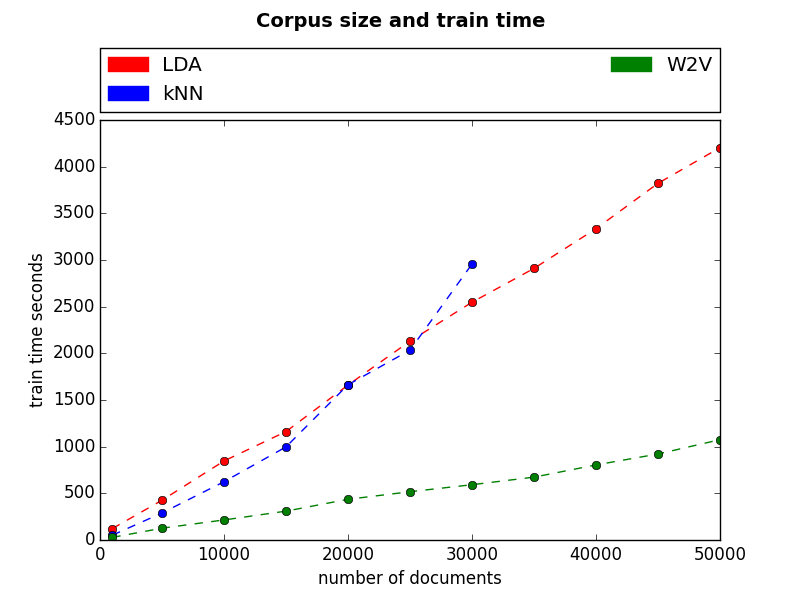
\includegraphics[width=0.7\textwidth]{Figures/TrainAll.png}
    \caption{Time to train LDA, k-NN, W2V}
    \label{fig:TrainAll}
\end{figure}

\subsection{Querying}
The querying of the recommendations was conducted by feeding 50 unseen documents into the models and logging the time taken to generate results.
The results from querying can be seen in Figure~\ref{fig:queryAll}.
As explained above, k-NN fails to create a model after approximately 30,000 documents.
For this reason there are no query results for k-NN after 30,000 documents.

\begin{figure}[h]
    \centering
        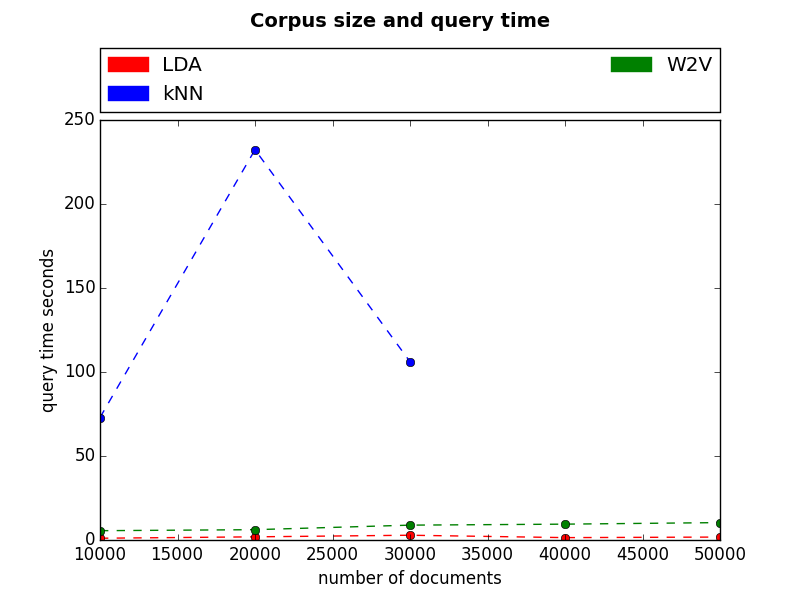
\includegraphics[width=0.7\textwidth]{Figures/queryAll.png}
    \caption{Time to query LDA, k-NN, W2V}
    \label{fig:queryAll}
\end{figure}

\section{Recomendation Performance}
The recommendation performance of LDA, k-NN and Word2Vec is split into two sections.
For the manual analysis a sample of the recommendations are selected and evaluated based on their quality.
The arXiv comparison has been conducted by comparing the generated recommendations against the arXiv defined topics.

The query corpus consisted of 50 unseen documents, the breakdown of which can be found in Table~\ref{table:queryBreakdown}.
These queries were used on the models generated above.
However, unlike the above models which were generated on a corpus of ranging from 5,000-50,000 documents, the queries were applied to corpora increasing in size by 10,000 starting at 10,000 and finishing at 50,000 documents.

\begin{table}[h]
    \centering
    \begin{tabular}{|c c|}
         \hline
         arXiv Topics & Number Documents \\ [0.5ex]
         \hline\hline
         astro-ph & 10 \\
         cond-mat & 10 \\
         cs & 10 \\
         math & 10 \\
         physics & 10 \\ [0.5ex]
         \hline\hline
         Total & 50\\ [1ex]
         \hline
    \end{tabular}
    \caption{Breakdown of papers from query corpus}
    \label{table:queryBreakdown}
\end{table}

\subsection{Manual analysis}
As each of the algorithms being investigated are unsupervised and there is no gold standard to compare their results against, a manual evaluation of the results must be conducted.
This involved selecting three papers from each of the five arXiv topics and evaluating the quality of the recommendations generated.
In total 15 papers were selected and the top five recommendations generated by each of the algorithms were evaluated based on their coherence to the query document.
This process is prone to tedium and it is possible that the person classifying the documents may be unable to identify similarities due to a lack of knowledge of a particular field.

\subsection{arXiv comparison}
Unlike the manual comparison, which can only evaluate a small number of results, this comparison uses the arXiv meta-data to compare against the recommendations generated.
This is also imperfect due to the meta-date only associating each document with one topic when it could in fact be on the edge of two different topics.

\section{Conclusion}
In this chapter the performance of LDA, k-NN and Word2Vec has been presented.
In temporal performance it was found that Word2Vec was the quickest at training a model of the corpus.
Word2Vec on the other hand generated quite poor recommendations and would not be useful for this purpose.
The k-NN library used generated passible recommendations but it was not able to scale above 30,000 documents and may be unsuitable in a real world context.
The temporal performance of the LDA grew linearly with the size of the corpus and was comparable to k-NN until it failed.
The results generated by LDA also seemed to be the most coherent recommendations.

In the following chapter I will present my conclusions from this research project and outline any possible future work that could be conducted.
